% !TEX root = main_org.tex

\newpage
\chapter{Jet energy loss as function of path-length}

\section{Basic motivation}

The nuclear modification factor, which is called $R_{AA}$, is one of the strong evidence of created medium in heavy ion collisions compare to $p+p$ collisions \cite{Adcox:2001jp}. In Quantum Chromodynamics(QCD), the suppression of high $p_T$ hadrons was predicted as the result of the energy loss of hard-scatters quarks and gluons in the hot and dense medium. 


\section{Analysis}
	\subsection{Inclusive $R_{AA}$}
	To compare heavy ion collisions to $p$-$p$ collision, the nuclear modification factor $R_{AA}$ is defined. 
	
  \begin{equation}
  R_{AA}(p_{T}) = \frac{(1/N^{evt}_{AA})dN^{AA}/dp_{T}}{ \langle N_{coll}\rangle(1/N^{evt}_{pp})dN^{pp}/dp_{T}}
  \end {equation} 
  \smallskip
  
  where $dN^{AA}/dp_T$ and $dN^{pp}/dp_T$ are the yields in heavy ion collisions and $p$-$p$ collisions, respectively. $ \langle N_{coll}\rangle$ is the average number of binary nucleon-nucleon collisions in one heavy ion collision event. 

 Without medium effect, the nuclear modification factor $R_{AA}$ should be 1. However, in heavy ion collision the nuclear modification factor is usually smaller then 1 \cite{Roland201470, PhysRevLett.101.232301, PhysRevLett.91.172302}. These suppression for the high $p_T$ hadrons can be explained by ``jet quenching'', and this is the one of probe for the existence of QGP medium. Compare with RHIC, LHC show a stronger modification  \cite{Roland201470}. This indicate an enhanced energy loss and hence a denser medium was produced at the LHC. 


	\subsection{Elliptic flow}
	Anisotropic flow is the well known feature in both theoretical and experiment in heavy ion collision. It provides the hints to understand collision evolution and thermalization process. (See section.\ref{sec:flow} for the details)
	\smallskip
 \begin{equation}
 \frac{dN}{d\Delta\phi}=\frac{x_0}{2\pi}+\frac{1}{2\pi}\sum_{n=1}{(2v_n\cos{n(\phi-\psi_n)})}
\end{equation} 
	\smallskip

The function of $\frac{dN}{d\Delta\phi}$ shows  the particle distribution in transverse direction.  This anisotropy particle production is known as flow effect. Especially, elliptical flow, which is second order flow $v_2$ is well explained by almond shape initial geometry. But the shape of the collision geometry is not a perfect almond shape because the collision nucleon is not uniform sphere. Therefore, the created medium is not homogenous and has complex shape.  These are the reason of flow fluctuation and cause of higher order flow. This higher order flow which comes from fluctuation and is not strongly affected by the centrality of the collision. Because the distribution of the participating nucleons in collision is totally random, so fluctuation is depends on event by event geometry and these effect will be minimized in average over events. 

	\subsection{$R_{AA}$ as function of $\Delta\phi$}
	  As the nuclear modification factor represent the ratio of yield of particle produced in heavy ion and $p$-$p$ collision, one can make $R_{AA}$ as a function of $p_T$ and $\Delta \phi$, where $$ \Delta \phi  = \phi - \psi_{n}$$ by using definition of flow. Since, the yield of $p$-$p$ collision does not have reaction plane, we can estimate the ratio of particle produced in $\phi$ angle is uniform over the event average. Therefore, the definition of $R_{AA}$ as function of $p_T$ and $\Delta \phi$ can be written as \cite{Liao:2009ni, Adler:2006bw}
    \begin{eqnarray}
  R_{AA}(p_{T}, \Delta \phi) &=& \frac{(1/N^{evt}_{AA})d^2N^{AA}/dp_{T} d\Delta\phi}{ \langle N_{coll}\rangle(1/N^{evt}_{pp})dN^{pp}/dp_{T}}\\
  &=& {R_{AA}(p_T)}\frac{dN^{AA}}{d\Delta\phi}\\
  &=& {R_{AA}(p_T)}(1+\sum_{n=1}{(2v_n\cos{n(\Delta \phi)})}
  \end {eqnarray}
\smallskip

  If we neglect high order flow which comes from fluctuations, above equation can be simplified like 
   \begin{eqnarray}
  R_{AA}(p_{T}, \Delta \phi) &\sim& {R_{AA}(p_T)} (1+2 v_{2} \cos{2\Delta \phi})
  \end {eqnarray}
\bigskip

	\subsection{Path-length calculation with Glauber model}
	
  If we assume all particles are produced from the center of collision region, then it is possible to represent path-length as function of centrality and $\Delta\phi$ which is transverse angle with respect to the reaction plane. To analyze the path-length dependence of $R_{AA}$, we estimate the path lengths of patrons in the medium as the distance from  the center to the edge of the elliptical overlap zone of the heavy ion collision(See Fig.\ref{Fig1}). To calculate this length, TGlauber Monte Carlo simulation has been used to evaluate  for all variations as function of impact parameter(centrality). of medium to the edge.  
  
\begin{figure}[htbp]
\begin{center}
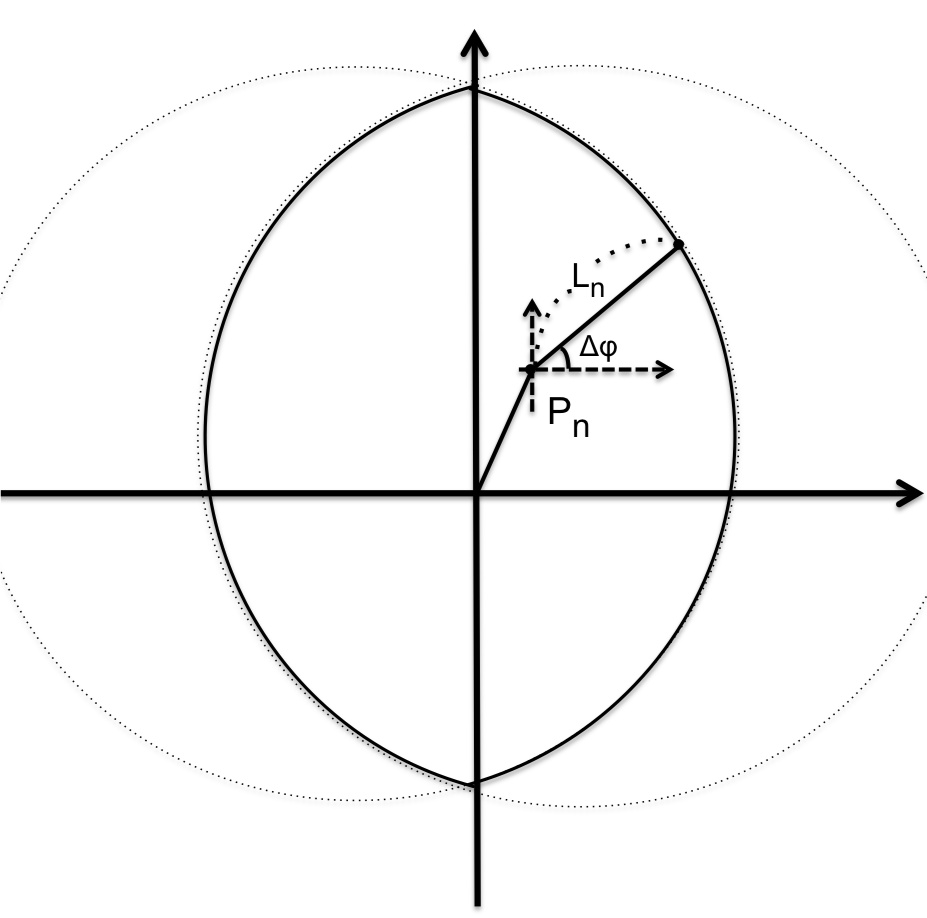
\includegraphics[height=5cm]{figures/Fig_pathlength/fig1.jpg}
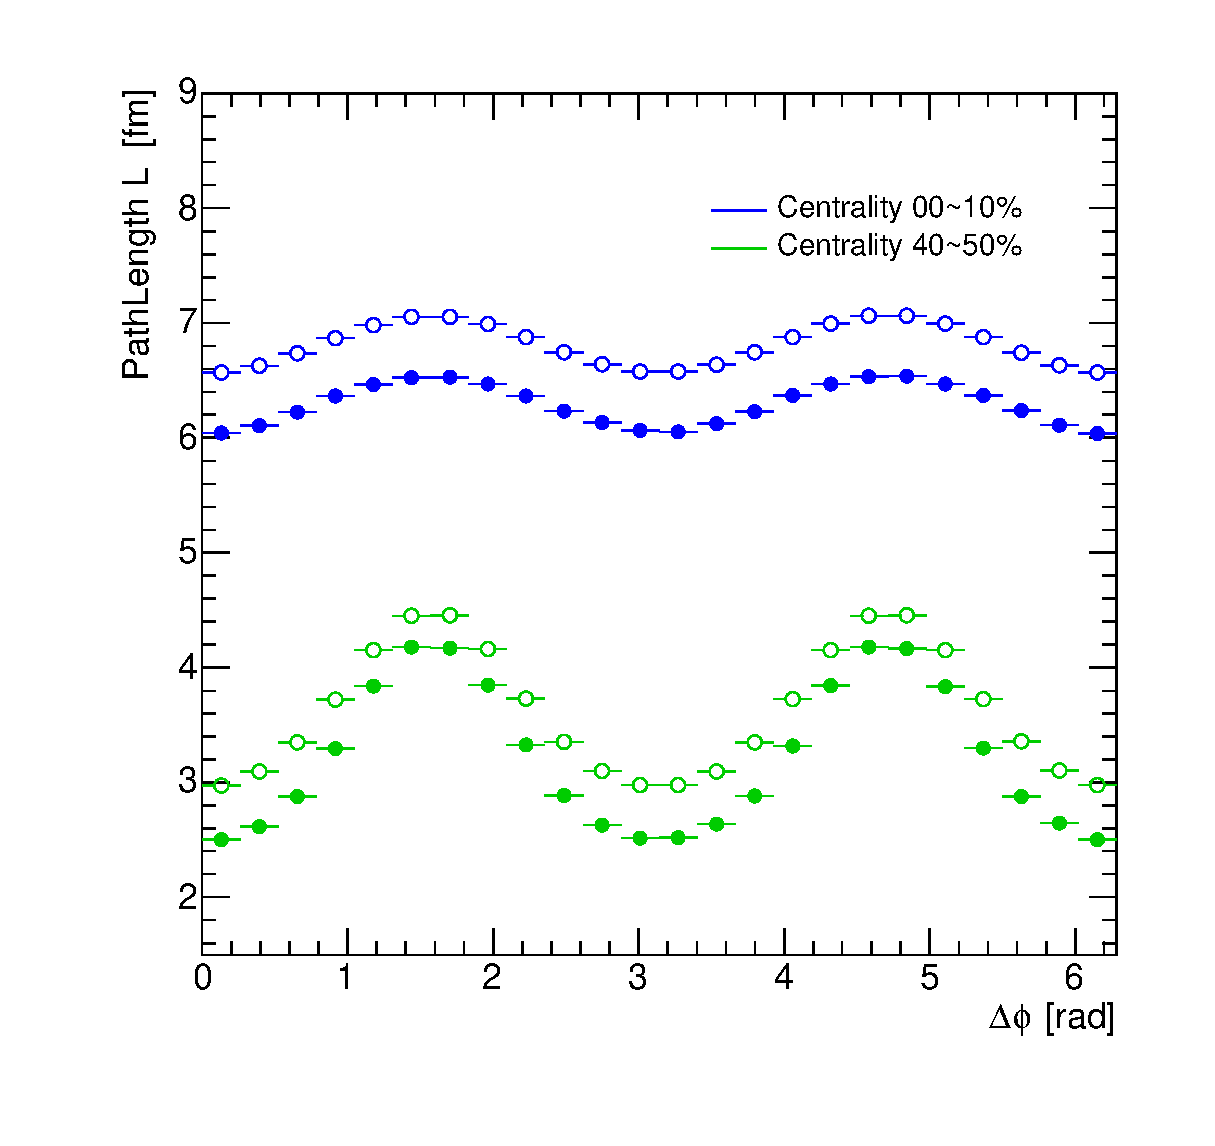
\includegraphics[height=5cm]{figures/Fig_pathlength/fig2.eps}
\caption{Basic concept of definition of path-length for given angle $\Delta \phi$(top), and results for centrality 00-10\% and 40-50\%(bottom). Open symbols are path-length which is calculated from Eq.\ref{eq:pathlength}. Closed symbols are length from center to edge of region.}
\label{Fig1}
\end{center}
\end{figure}

  
   However, in  real situation, hard scattering happens in any collision point, also the direction where the parton travels is random. One would calculate a weight factor for the parton to travels into the divided region we set. In this case, proper path length is the average value of length from the collision points to the edge of collision region for given angle, such as
   
 \begin{equation}
L(\Delta \phi)=\frac{\Sigma_{n=1}^{N}{Ln(\Delta \phi)}}{N}
\label{eq:pathlength}
\end{equation}
 where N is number of binary collisions, and $L_{n}(\Delta \phi)$ is length from $n_{th}$ collision point($P_n$ in Fig.\ref{Fig1}) to edge of collision shape for given angle $\Delta \phi$.  This length is always longer then length from center to edge of collision region.
 


\section{Result}
	\subsection{$R_{AA}(p_T, \Delta\phi)$}
	For LHC experiment, the Nuclear modification factor, $R_{AA}$, of the Pb-Pb values has been published by ALICE collaboration\cite{Abelev:2012hxa}. In Central collisions the field is most suppressed with $R_{AA}\sim0.13$ at $p_T=6\sim7$GeV/$c$. Above $p_T >$ 7 GeV/$c$, there is a significant rise in the nuclear modification factor for $p_T >$ 30 GeV/$c$.  In peripheral collisions, the suppression is weaker with $R_{AA} \sim 0.7$ and not much dependence of $p_T$. Also the flow values $v_n$ has been measured by CMS collaboration\cite{Chatrchyan:2012ta} up to $p_T=20$GeV/$c$ for each centrality for same collision energy for Pb-Pb. They measured elliptic flow(in terms of Fourier components of the azimuthal distribution, the n=2) with using unidentified charged particles in $|\eta| < 2.4$. The anisotropic flow values are maximized around intermediated $p_T \sim 4GeV/c$. To facilitate a quantitative comparison of there result, the CMS measurements are fitted with a combination of a fifth-order polynomial function (for $p_T < 4.2GeV/c$) and a Landau distribution (for $p_T > 4.2$GeV/$c$). The Results are shown in Fig.\ref{apendfig2}, there is almost a factor of 2 or more suppression out-of-plane(where $\Delta \phi = \pi /2 $) than in-plane( $\Delta \phi = 0 $) near $p_T = 3$GeV/$c$ in Centrality 20\% to 30\%. This suppression goes down when $p_{T}$ moves higher. 
\begin{figure}[htbp]
\begin{center}
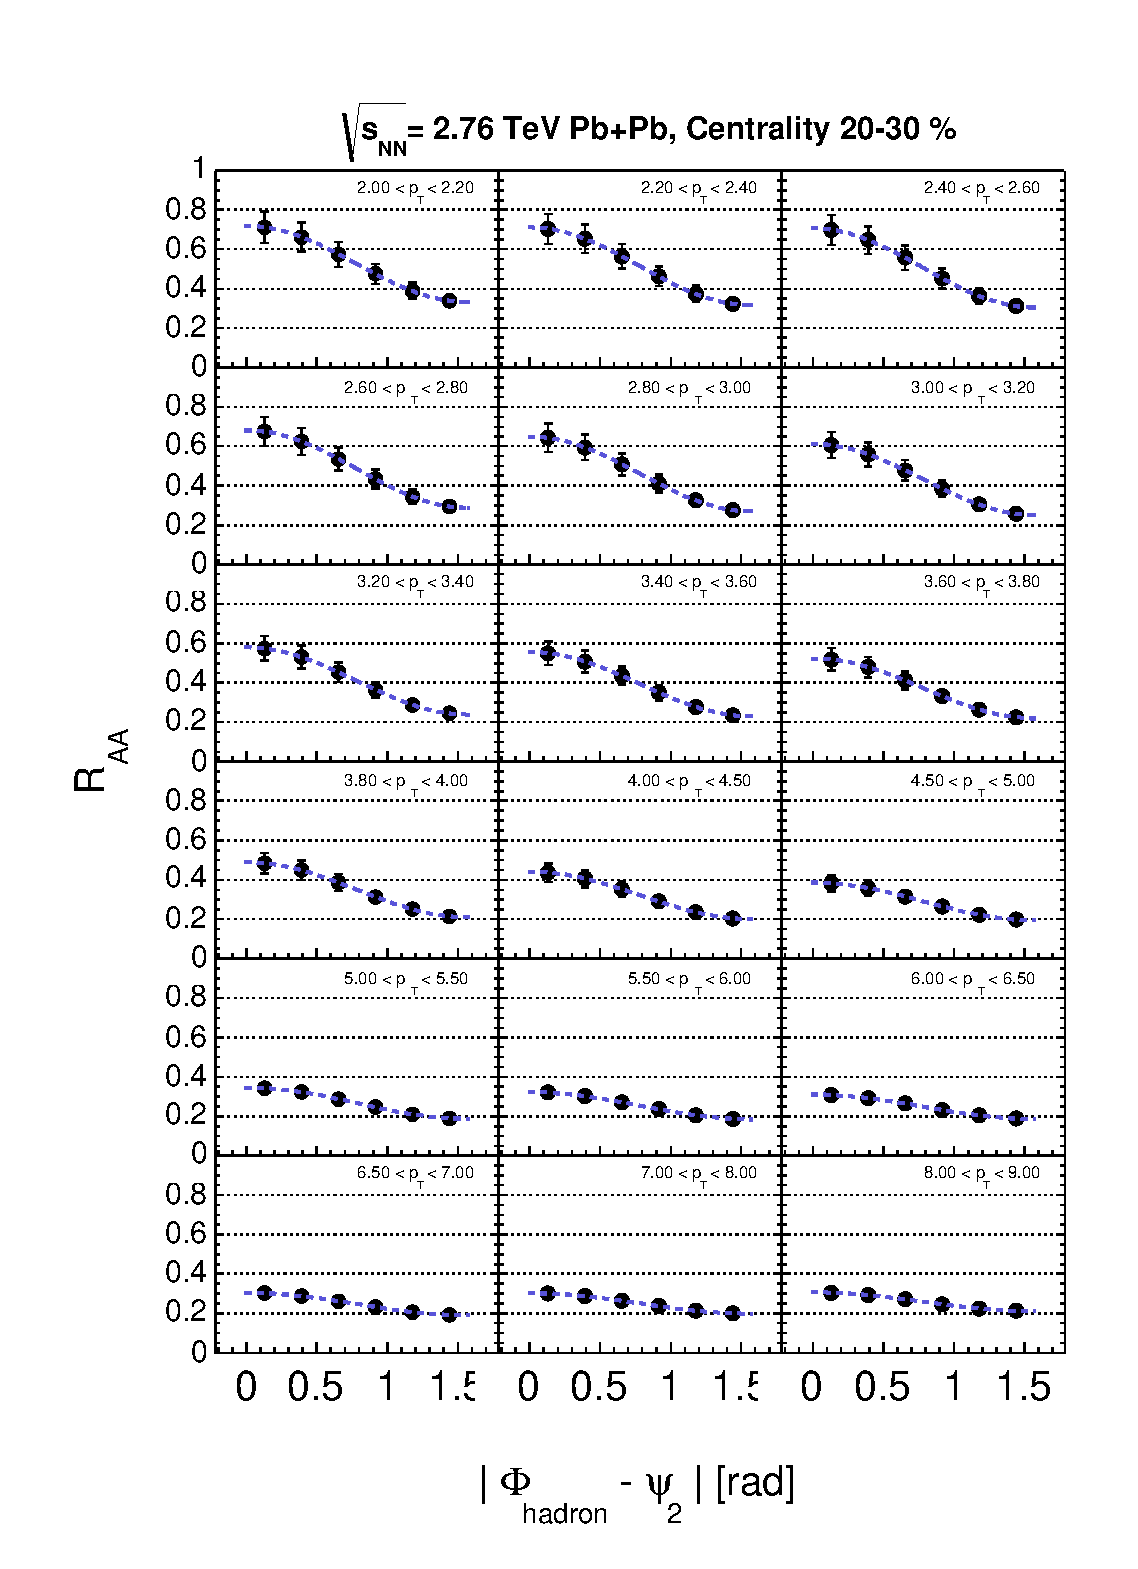
\includegraphics[height=15cm]{figures/Fig_pathlength/fig3.eps}
\caption{$R_{AA}$ versus $\Delta \phi$ for LHC experiment for given $p_{T}$ bins. Statistical errors and systematical errors are evaluated quadratic.}
\label{apendfig2}
\end{center}
\end{figure}
For RHIC experiment, the $R_{AA}$ values as function of $\Delta \phi$ of neutral pion with respect to centrality in Au+Au collisions at $\sqrt{S_{NN}}= 200GeV$ has been Published by PHENIX collaboration. \cite{Adare:2012wg}


	\subsection{Convert $\Delta\phi$ to path-length}
	By using TGlauber simulation\cite{Alver:2008aq}, for each Pb+Pb with collision energy 2.76TeV and Au+Au with collision energy 200GeV, the path length estimation has been done. To get average values of length between collision point to outside of shape, divide by 6 bins(0$\sim$15, 15$\sim$30, 30$\sim$45, 45$\sim$60, 60$\sim$75, 75$\sim$90 degree) and find outermost wounded nucleon for each bins. Then histograms are filled with length from collision point to outermost nucleon and its transverse angle. The averaged values as path length for given angles are shown in Fig.\ref{apendfig3}

\begin{figure}[!h]
\begin{center}
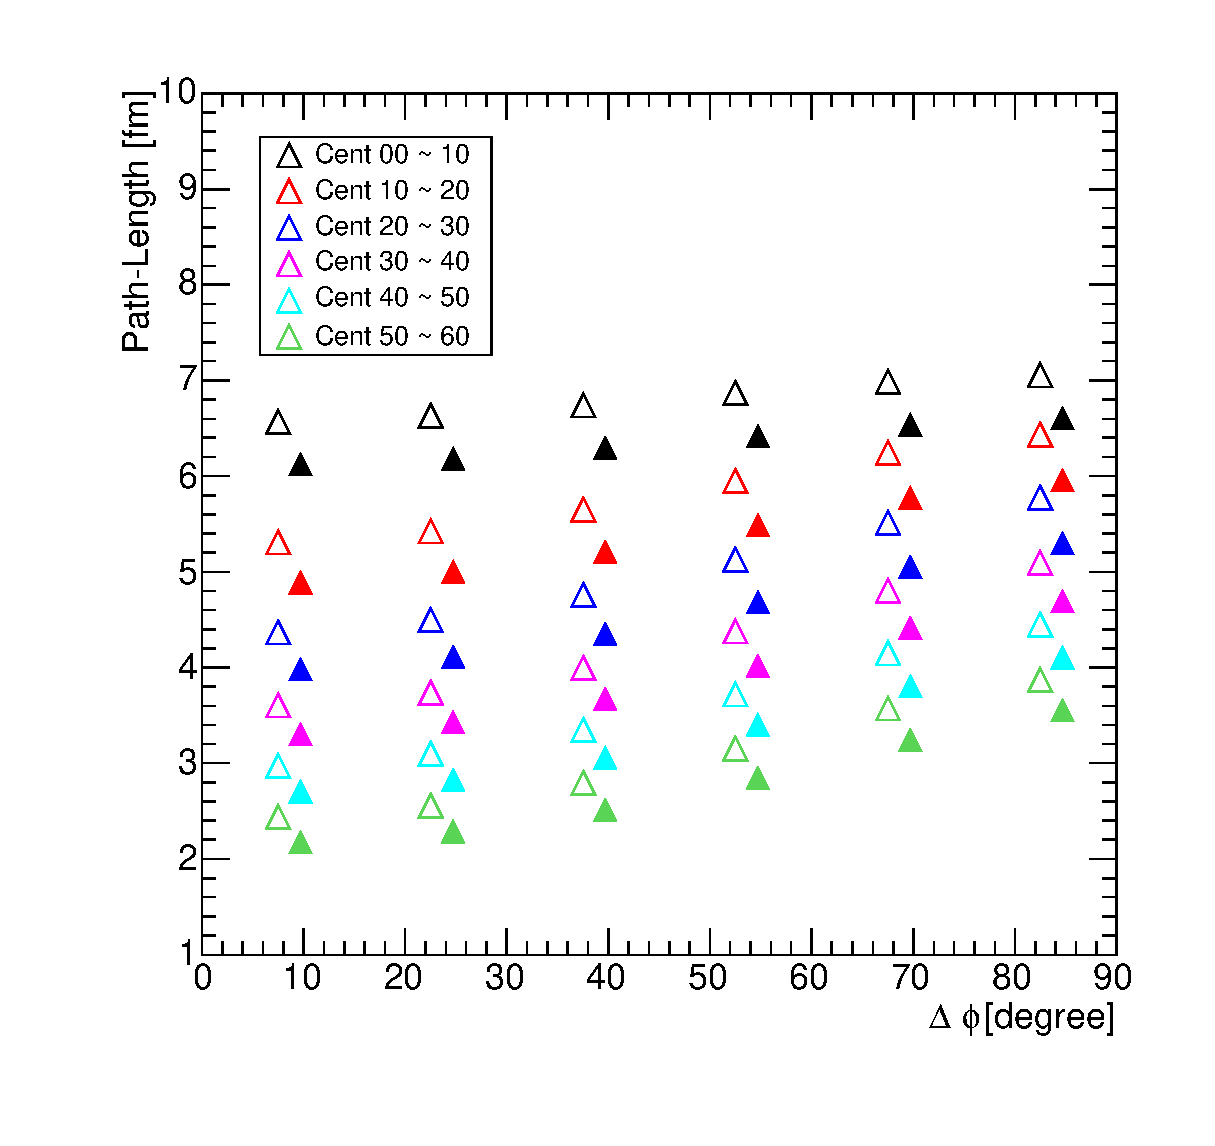
\includegraphics[height=8cm]{figures/Fig_pathlength/fig9.eps}
\caption{Geometrical simulation result of path length calculation vs angle with respect to reaction plane by using TGlauber simulation for ALICE(open symbols) and PHENIX(closed symbols), plotted for the six centralities as shown in legend. The angle respect to reaction plane, $\Delta \phi$ is for the center of the bins(7.5, 22.5, 37.5, 52.5, 67.5 and 82.5) and centrality dependent offset is introduced for visual clarity }
\label{apendfig3}
\end{center}
\end{figure}

Based on Glauber simulations, there is no apparent path-length change in central collision. In peripheral regions, the path length has been changed more then 10\% and, Path-length of out-of-plane is even longer then path-length of in-plane in more central collisions. For example, the path-length of out-of-plane in 30\%$\sim$40\% is approximately equal to the path-length of in-plane in 20\%$\sim$30\% centrality classes. The ALICE simulation result has always slightly longer path-length then PHENIX because of size of heavy ion species



\begin{figure}[htbp]
\begin{center}
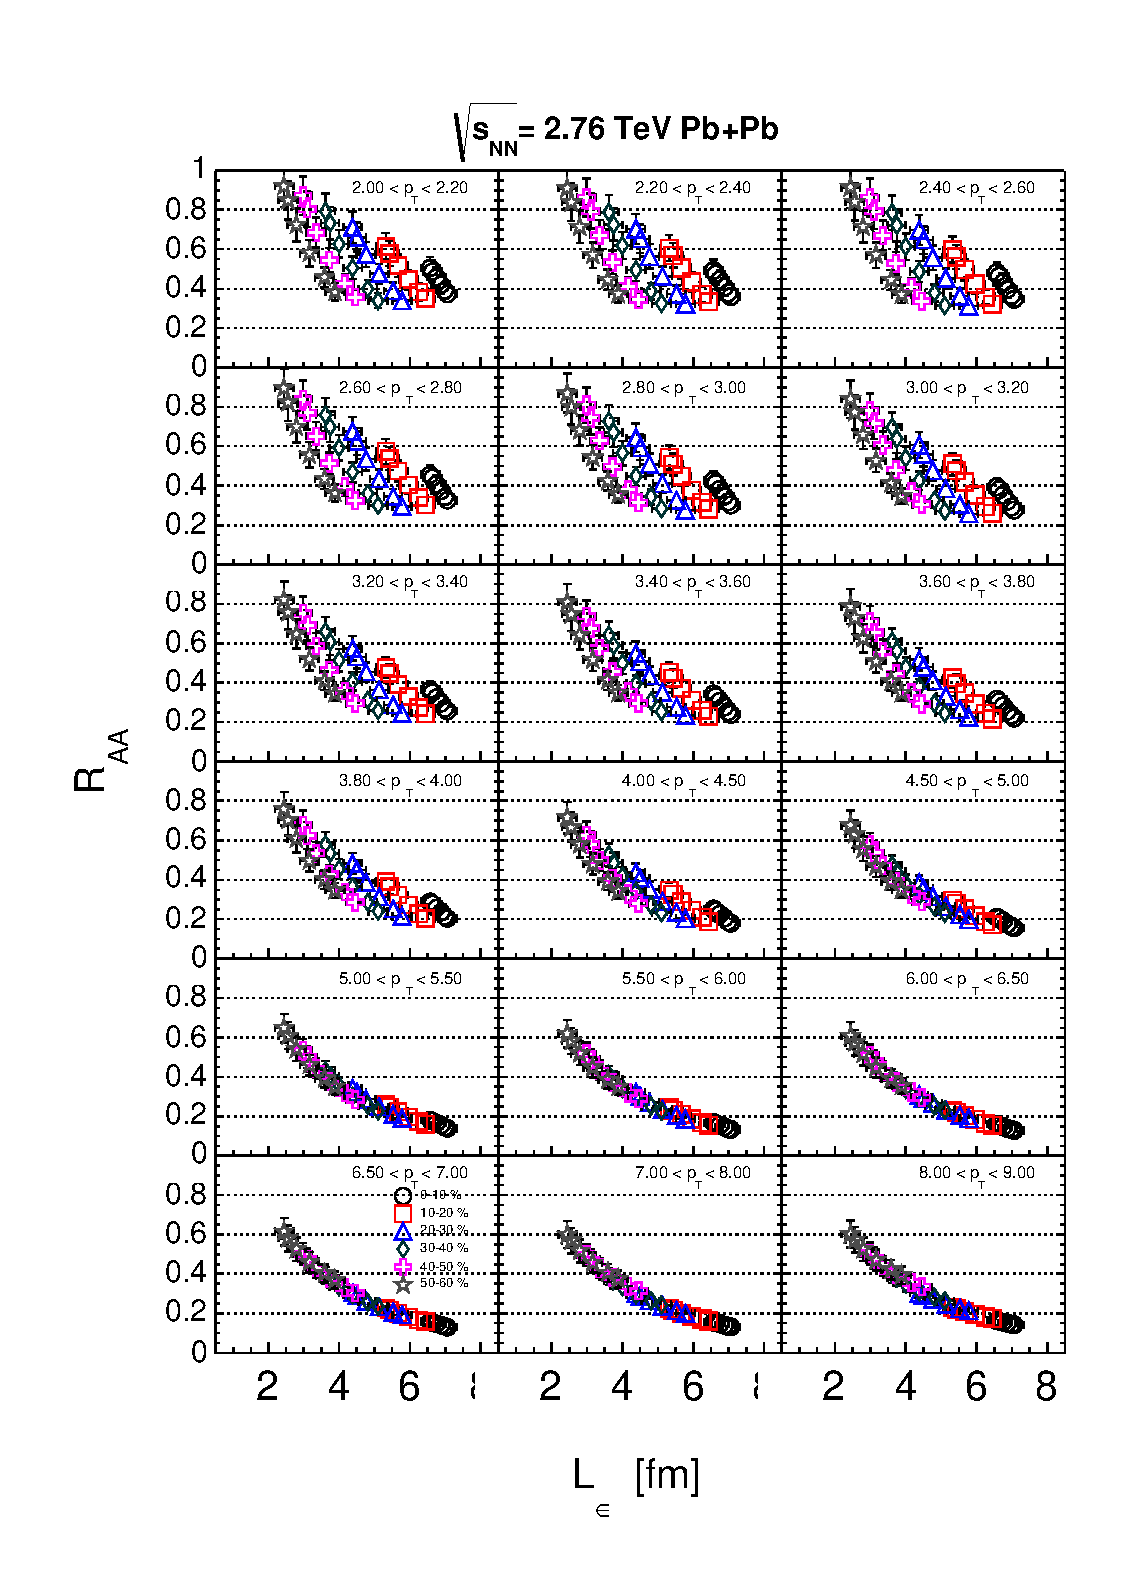
\includegraphics[height=10cm]{figures/Fig_pathlength/fig4.eps}
\caption{ $R_{AA}$ versus Path-length correspond to $\Delta \phi$ for LHC experiment for given $p_{T}$ bins. Statistical errors and systematical errors are evaluated quadratic. }
\label{apendfig4}
\end{center}
\end{figure}

	\subsection{Path-length dependence of $R_{AA}$}
	As a result, the $R_{AA}$ values as function of $\Delta \phi$ are converted to as function of path length for each centralities. For given centrality, variation of $\Delta \phi$ gives a variation of the path length transversed for fixed initial conditions. Fig.\ref{apendfig4} shows the nuclear modification factor $R_{AA}$ as a function of path-length for each $p_{T}$ bins for LHC experiment. The results indicate that the suppression depends on the path-length for high $p_T$ region particles. For the $p_T > 5GeV/c $bins, the slopes in the individual centralities are aligned together. And $R_{AA}$ seems universal function with path length L for all centrality classed for $p_T > 5GeV/c$ ranges within errors.  To compare with PHENIX result, the same $p_T$ bin has been chosen and shows in Fig.\ref{apenfig5}. Both result are fitted by following function
\begin{equation}
\frac{a}{a+L^n}
\end{equation}
where, a is arbitrary constant and L is path length. With this function we expect $R_{AA}= 1$ at path-length L = 0, and $R_{AA} = 0$ at path length $L = \infty$. For all centralities with more then $p_T > 5GeV/c$, the function works well with  $ n \sim 2 $ for both result.


\begin{figure}[htbp]
\begin{center}
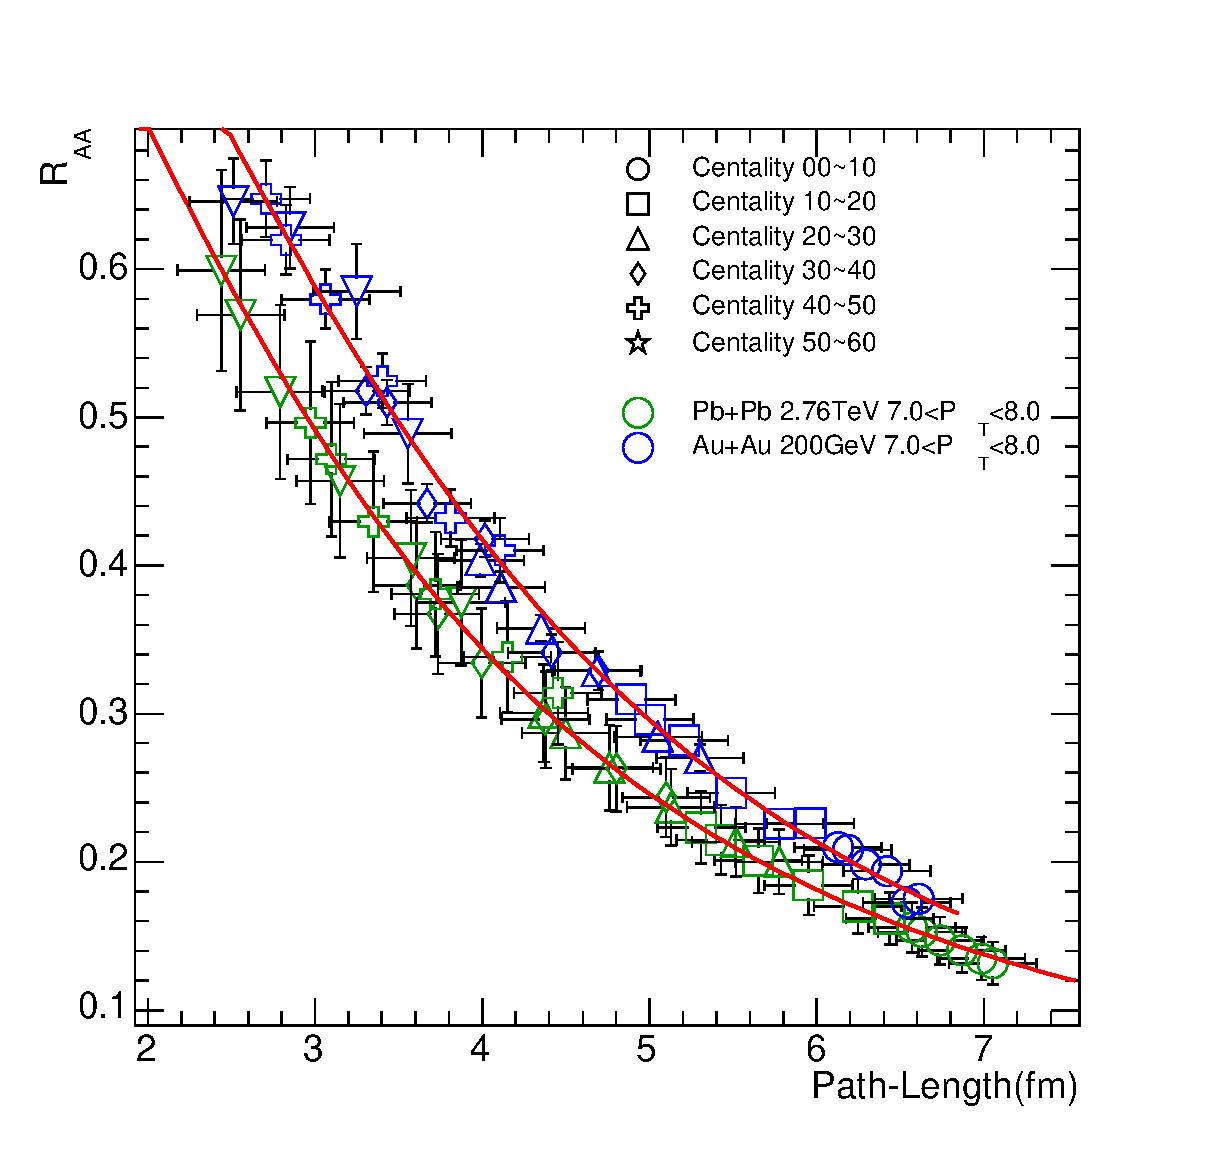
\includegraphics[height=7cm]{figures/Fig_pathlength/fig10.eps}
\caption{Comparison of $R_{AA}$ as function of path length for ALICE and PHENIX with 7$\sim$8 GeV/$c$ $p_T$ bin  }
\label{apenfig5}
\end{center}
\end{figure}



\section{Summary}

One of the prediction of parton energy loss calculation is the average energy loss can be represent as a function of the mean free path in medium. And energy loss in medium can be indirectly evaluated from nuclear modification factor, $R_{AA}$. With combination of using inclusive $R_{AA}$ and flow, we can estimate the dependence of suppression on geometry which related to mean free path length. we presented result of path-length dependence of $R_{AA}$ by using flow harmonics and calculation of path length from glauber simulation. As the results, in high $p_T$ ranges ($p_T > 5.0$ GeV/$c$), the $R_{AA}$ seems universal function with path length. Moreover the decrease slope of $R_{AA}$ as function of path-length were well fitted by 2nd order inverse function.